\chapter{ISTTOK }

ISTTOK is a large aspect ratio tokamak (IPFN-IST, Lisbon, Portugal) operating for 30 years and which has been in constant upgrading of diagnostics, hardware acquisition system and control algorithms (major and minor plasma radius are respectively $R= 46 \, cm$, $a= 8.5 \, cm$). Together with the JT60-SA development of control techniques from last chapter, ISTTOK  studies  complement as a whole this work. This chapter will detailed how ISTTOK operates, from topics such as describing its diagnostics to description of the reconstruction method for calculating the plasma centroid position.

\section{Machine description}

The construction  of the actual ISTTOK machine was started in 1990 reusing some parts of the former dutch TORTUT tokamak: support structure, vacuum vessel, copper shell, toroidal magnetic coils, transformer, capacitor banks, radiofrequency (rf) generator, and discharge cleaning system ~\cite{Varandas1996}. The toroidal magnetic field is given by a set of 24 conventional coils which generate a maximum of 3~ T. The other components of ISTTOK such as the vacuum systems, the PF coils, and the power supply for the toroidal magnetic coils,  as well as its diagnostics and control and data acquisition system, were locally designed and built. Figure ~\ref{TopISTTOK} shows a top view of the ISTTOK tokamak and figure~\ref{ISTTOK_front} a frontal one in early 2020, its main elements are signalized with arrows.\smallskip

\begin{figure}[htbp]
	\centering
	\includegraphics[width=1.1\textwidth]{Chp4/TopISTTOK.png}
	\caption{\label{TopISTTOK} ISTTOK top view in 2020,   main elements are indicated with magenta  lines.}
\end{figure}

\begin{figure}[htbp]
	\centering
	\includegraphics[width=1.1\textwidth]{Chp4/FrontISTTOK.png}
	\caption{\label{ISTTOK_front}ISTTOK frontal view in 2020, main elements are indicated with blue lines.   }
\end{figure}

Figure ~\ref{VV_IST} corresponds to a section of the ISTTOK vacuum vessel, it is possible to observe on the image the ribbed  surface from the vessel and some of the ports on the top of it. The vacuum vessel is formed by two half torus made of INCONEL alloy 625 with a thickness of 0.15~ mm. The vacuum vessel is completely surrounded by a 1.5 ~cm thick cooper shell which is possible to see in the images from figure~\ref{ISTTOKviews}, this shell supports the vacuum vessel and it originally  also worked suppressing  variations of the plasma position in less than 2~ms since a first version of TORTUR had no PF coils, this was a form of auto-control. The  cooper shell, due to its properties, adds a delay or skin time for the  penetration of the magnetic fields into the vacuum vessel.
\smallskip

\begin{figure}[htbp]
	\centering
	\includegraphics[width=0.65\textwidth]{Chp4/VacuumVessel_Low.png}
	\caption{\label{VV_IST} Actual ISTTOK inconel  vaccum vessel section with ports.  }
\end{figure}


One of the main characteristics from ISTTOK  is that due to the flexibility of the power supplies it is possible  to perform  AC  discharges  which  allow the fast reversal of the plasma current while maintaining a finite plasma density between consecutive flat tops  ~\cite{density}. The current inversions make it possible to achieve a much longer plasma duration in comparison to single mode operation, which is limited by the saturation of the iron core magnetization,the plasma duration is of approximately 1 s (~\cite{Fernandes1998}, ~\cite{Carvalho2015}~).







\section{Diagnostics and Actuators}

Different  diagnostics are integrated in ISTTOK to retrieve important plasma parameters, i.e. langmuir probes, tomography, magnetic probes. This work is focused on the magnetic diagnostics  since they are responsible for  retrieving the signals necessaries to reconstructed the centroid position of the column and the plasma current. ISTTOK has a set of 12 of magnetic  probes or Mirnov coils positioned along the poloidal direction, each coil has an area of $49 ~mm^2$ and 50 turns, a scheme is depicted in figure ~\ref{MirnvC}. Picture from figure ~\ref{MirnPort} shows the vessel side port where the magnetic probes are  placed and its acquisition cables along with some of the PF coils cables in orange and white. Each coil is inside a graphite box and the set of 12 forms the plasma limiter, see figure \ref{MirnvC_photo}. 
\smallskip



\begin{figure}
	\centering
	\begin{subfigure}[b]{0.37\textwidth}
		\includegraphics[width=\textwidth]{Chp4/MirnovCoil_locations_ISTTOK.eps}
		\caption{ Set of 12 magnetic probes for the reconstruction of the plasma centroid position located along the poloidal direction at ISTTOK.\label{MirnvC} }
	\end{subfigure}
	~~
	\begin{subfigure}[b]{0.37\textwidth}
		\includegraphics[width=\textwidth]{Chp4/MirnovCoil_locations_ISTTOK.eps}
		\caption{\label{MirnvC_photo} 3D model of ISTTOK magnetic probe coil }
	\end{subfigure}
	
	\caption{ \label{} }
\end{figure}



A second set of diagnostics important for this work are the three current transducers, also called LEMs, installed in ISTTOK for measuring the current applied by the power supplies  to each  PF coils, figure ~\ref{LEM} show a picture of one LEM.

\smallskip


\begin{figure}[htbp]
	\centering
	\includegraphics[width=0.4\textwidth]{Chp4/LEM.png}
	\caption{\label{LEM} LEM transducer for measuring the current from the power supplies to the PF coils.  }
\end{figure}

\begin{figure}
	\centering
	\begin{subfigure}[b]{0.37\textwidth}
		\includegraphics[width=\textwidth]{Chp4/PuertoMirnov.png}
	\caption{\label{MirnPort}Magnetic probes port with connection cable to the ATCA acquisition boards, also PF coils and cooper shell are shown. }
	\end{subfigure}
~~~~
	\begin{subfigure}[b]{0.37\textwidth}
		\includegraphics[width=\textwidth]{Chp4/PFCoils.png}
	\caption{\label{ISTTOKpfCoils}PF coils close up,primary coils correspond to the  white cables and vertical and horizontal to the orange ones. }
\end{subfigure}

 \caption{ISTTOK close up side views. \label{ISTTOKviews} }
 
 
\end{figure}

\subsection{Poloidal Field Coils}

ISTTOK poloidal field coils are placed in between the TF coils and the cooper shell. In figures ~\ref{MirnPort} and ~\ref{ISTTOKpfCoils} is possible to see the cables from the PF coils arrange in sets of orange and white cables. ISTTOK Poloidal Field (PF) coils are connected to three independently feedback controlled power supplies for the purpose of generating plasma current and also to control vertically and horizontally its centroid position. The primary PF coils, in white color, generate ohmic heating for the creation of plasma current and an additional vertical field. In figure~\ref{PF_coils} is shown on the right side of the iron core an  old central solenoid which used to be responsible for plasma current generation, this element is currently disconnected.  In yellow is depicted the vertical PF coils and in green the horizontal PF coils, both controlled by different control algorithms in order to follow a centroid position set point \cite{IvoPID}. Figure ~\ref{PF_lines} shows the magnetic field lines generated by each PF coil around the vacuum chamber cross section on their nominal positions.
\smallskip


%% Aqui va la figura de Dori
\begin{figure}[htbp]
	\centering
	\includegraphics[width=0.85\textwidth]{Chp4/ist_coils.eps}
	\caption{ 3D scheme of the ISTTOK PF coils, vacuum chamber with ports, iron core and the former central solenoid (black color) . Primary coils (white color) and horizontal coils (green color) are formed by 2 coils each one and located on the  upper and lower LFS (Low Field Side) of tokamak. Vertical coils (yellow color) are formed by 4 coils, 2 are located on the upper and lower LFS and 2 in the upper and lower HFS (High Field Side). Figure 26 in section 1.5 of ref. \cite{Ivo}. \label{PF_coils}  }
\end{figure}

\begin{figure}[htbp]
	\centering
	\includegraphics[width=1.12\textwidth]{Chp4/PF_fieldLines.png}
	\caption{ Magnetic field generated by the active coil circuits on their nominal positions. Mirnov positions are represented by its sequential number (in red) over the dashed line. Black circle represents the limiter.\label{PF_lines}  }
\end{figure}


%The ohmic heating (OH) coils of the tokamak transformer,
%Since the ISTTOK central solenoid is not being used as the primary winding to create the toroidal electric field responsible for creating and maintaining the plasma current  $I_p$ ,

As mentioned before, figure~\ref{PF_coils} shows the  nominal positions of the PF coils .





\section{ISTTOK Hardware }

ISTTOK real-time control diagnostics and actuators  implementation rely  on the recently upgraded hardware based on the Advanced Telecommunications Computing Architecture (ATCA).   The real-time control system is programmed on top of the Multi-threaded Application Real-Time executor (MARTe) framework,  which  integrates and processes the information gathered by all the  diagnostics \cite{Ivo2}, figure ~\ref{ISTTOK_hard} depicts the schematic of the implemented control system at ISTTOK.

\begin{figure}[htbp]
	\centering
	\includegraphics[width=0.85\textwidth]{Chp4/control_schem_1.PNG}
	\caption{\label{ISTTOK_hard} ISTTOK hardware overall scheme. Data is acquired by the
		ATCA data acquisition boards, and decimated and transferred to the hosts
		every 100 $~\mu s$. }
\end{figure}


Recently implemented hardware-integrated acquisition of the magnetic probes signals at ISTTOK allowed the implementation of new real-time algorithms for an accurate reconstruction of the current centroid position. \smallskip

\subsection{ATCA-MIMO-ISOL boards}

The ATCA carrier board, already slightly address in chapter ~\ref{Chap2}, is an IPFN developed board ~\cite{Batista2010} complying with the ATCA standard specification, highly modularized, and with an optional Rear Transition Module (RTM) . The carrier board can hold up 32 analog input channels, each connected to a plugged-in ADC module. All modules are connected digitally to a XILINX Virtex-4 FPGA which performs necessary digital signal processing and includes a PCI Express Endpoint providing the data interface to the ATCA switch board.
\smallskip

\section{Real-time  integration software}

To recover the magnetic fields absolute magnitude from inductive probe signals an integrating component is needed. Typical analog electronic integrator circuits always suffer from voltage offsets and drifts present in the components and wiring. Even very low offsets integrated during a long period of time may appear as a noticeable deviation of the integrated signals ~\cite{Spuig2003} and eventually saturate their outputs. 
\smallskip

\begin{figure}[htbp]
	\centering
	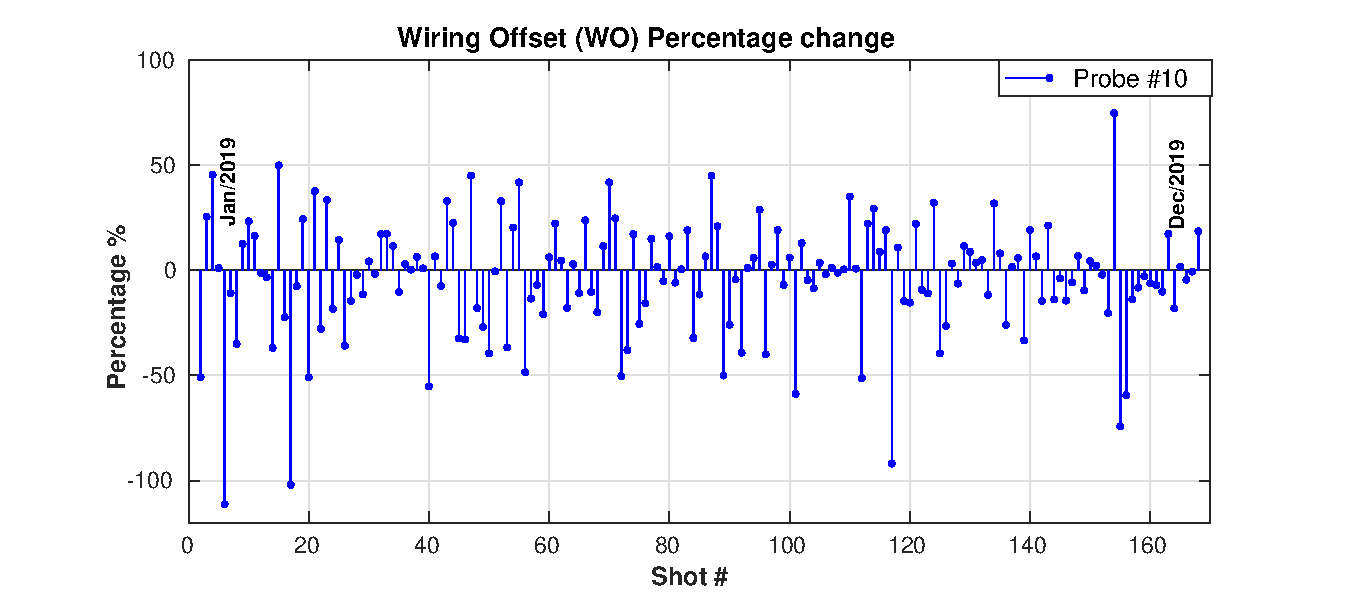
\includegraphics[width=0.85\textwidth]{Chp4/percentage_change.eps}
	\caption{\label{WO_percent}  }
\end{figure}

\begin{figure}[htbp]
	\centering
	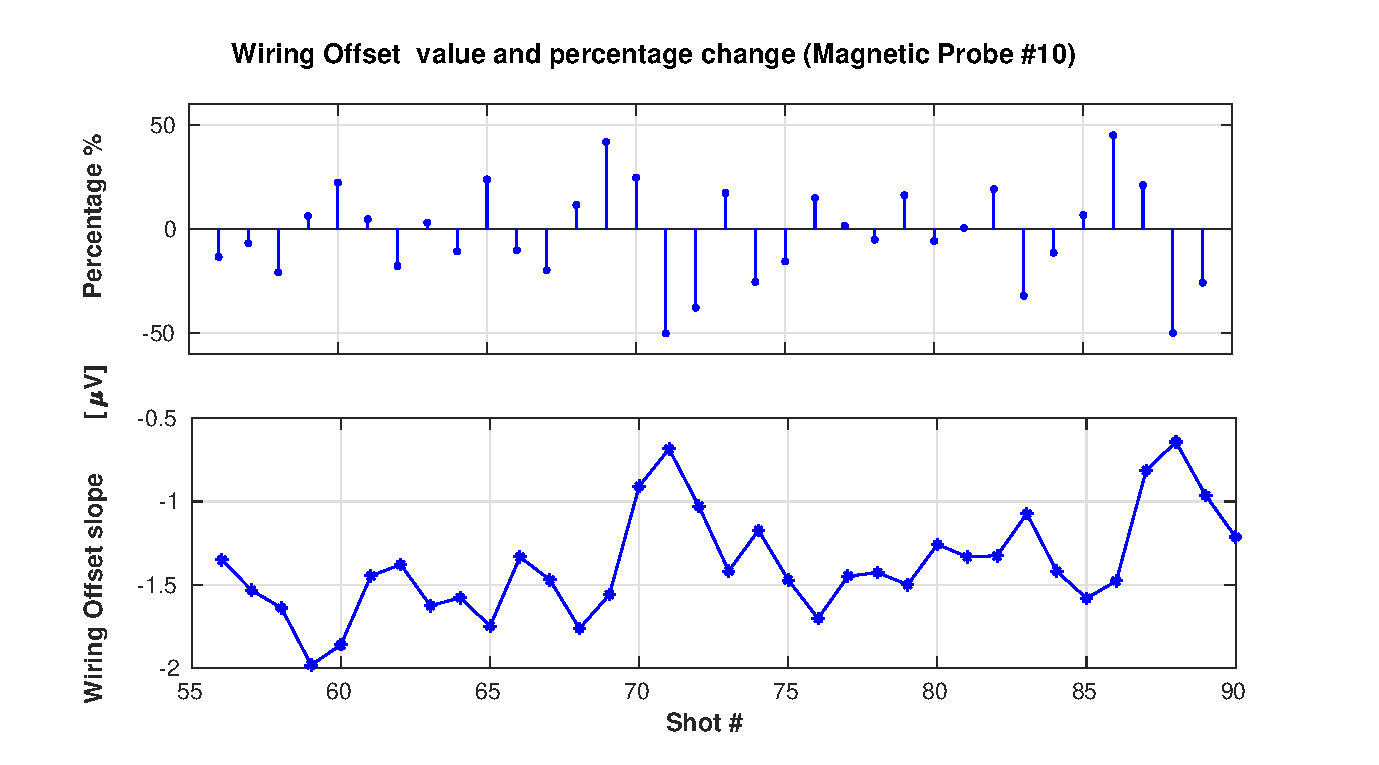
\includegraphics[width=0.85\textwidth]{Chp4/valueAndpercentage_change10.eps}
	\caption{\label{WO_minr10}  }
\end{figure}


Relying  on the flexibility of MARTe and the ATCA boards in ISTTOK it is possible to acquire data even thought this signals before the discharge takes place are not  stored on the data base, this feature allows to compute the WO of each probe several seconds before the discharge starts. GAM


\section{Plasma current magnetic field }

Performing plasma-less discharges in ISTTOK by applying different step functions waveforms in the PF coils currents,  data-driven discrete state-space models were obtained in order to determine the contribution to the probes signals from passive-structures eddy currents and PF coils fluxes at any instant.\smallskip

Retrieving the contribution of the plasma current in tokamaks ...

The methods of correction of the magnetic error fields due to inaccuracies
of tokamak manufacturing and assembly are considered. The problems of the
plasma position and shape reconstruction based on magnetic field measurements are discussed.

\section{Plasma centroid position determination}

The vertical and radial plasma position centroid is an essential measurement  since must be computed on real-time so they are the input variables for the ISTTOK control position.
